% Created 2017-09-21 Thu 21:31
% Intended LaTeX compiler: pdflatex
\documentclass[11pt]{article}
\usepackage[utf8]{inputenc}
\usepackage[T1]{fontenc}
\usepackage{graphicx}
\usepackage{grffile}
\usepackage{longtable}
\usepackage{wrapfig}
\usepackage{rotating}
\usepackage[normalem]{ulem}
\usepackage{amsmath}
\usepackage{textcomp}
\usepackage{amssymb}
\usepackage{capt-of}
\usepackage{hyperref}
\usepackage{amsmath}
\author{Jake Brawer}
\date{\today}
\title{Assignment 2}
\hypersetup{
 pdfauthor={Jake Brawer},
 pdftitle={Assignment 2},
 pdfkeywords={},
 pdfsubject={},
 pdfcreator={Emacs 25.2.1 (Org mode 9.1)}, 
 pdflang={English}}
\begin{document}

\maketitle

\section*{Problem 1}
\label{sec:org4d6bbb3}
\begin{equation}
f_{X}(X) = {{n}\choose{X}}\theta^{X}(1-\theta)^{n-X}
\end{equation}
\text{Finding the max here is tantamount to setting the derivative equal to 0 and solving for $\theta$:}\\

\begin{align}
  0 &= f_{X}'(X)\\
    &=  X{{n}\choose{X}}\theta^{X - 1}(1-\theta)^{n-X} - (n-X){{n}\choose{X}}\theta^{X}(1- \theta)^{n-X-1}
\end{align}
$\text{From here we get:}$
\begin{align}
    &(n-X){{n}\choose{X}}\theta^{X}(1- \theta)^{n-X-1} = X{{n}\choose{X}}\theta^{X - 1}(1-\theta)^{n-X}\\
  &(n-X)\theta^{X}(1-\theta)^{n-X-1} = X\theta^{X-1}(1-\theta)^{n-X}\\
  &(n-X)\theta(1-\theta)^{n-X-1} = X(1-\theta)^{n-X}\\
  &(n-X)\theta= X(1-\theta)\\
  &\theta n - \theta X = X - \theta X\\
  &\theta = \frac{X}{n}
\end{align}

\section*{Problem 2}
\label{sec:orgef92308}

\subsection*{A)}
\label{sec:org22cd0b1}
Let \(A\) be the event that both children are girls. let B be the event that at least one child is a girl.\\
Need to calculate $$P(A|B)$$

By Bayes theorem we have:
\begin{equation}
  P(A|B) = \frac{P(B|A)P(A)}{P(B)}
\end{equation}

By logic we know that $$P(B|A) = 1$$ so this simplifies to:\\
\begin{equation}
    P(A|B) = \frac{P(A)}{P(B)}
  \end{equation}
  \text{It is clear that $P(A) = \frac{1}{4}$ and $P(B) = \frac{3}{4}$ so:}\\
\begin{equation}
  P(B|A) = \frac{1}{3}
\end{equation}

\subsection*{B)}
\label{sec:org1c9e3de}
Let \(A\) be the event that both children are girls. let \(B\) be the event that at least one child is a girl. Let \(C\) be the event of being born on Tuesday.\\

Need to calculate $$P(A|BC)$$

By Bayes theorem we have:
\begin{equation}
  P(A|BC) = \frac{P(BC|A)P(A)}{P(BC)}
\end{equation}


The trick here is in calculating \(P(BC|A)\), which is the probability that at least one girl is born on Tuesday, given that both children are girls. There are \(49\) possible pairs of weekdays that these girls can be born on, \(13\) of which have at least one Tuesday. Thus $$P(BC|A) = \frac{13}{49} = .2653$$.

so:\\
\begin{align}
P(A|BC) &= \cfrac{\frac{13}{49}\frac{1}{4}}{\frac{1}{7}\frac{3}{4}}\\
&=\frac{13}{21}\\
&=.619
\end{align}

\subsection*{C)}
\label{sec:org503bcad}

The answer is the same as B), except \(P(C) = \frac{k}{7}\) and \(P(BC|A) = 1 - \frac{(7-k)(6-k)}{49}\)


\section*{Problem 3}
\label{sec:org45692c9}
\subsection*{A)}
\label{sec:org12b0390}

\emph{To prove}: $$P(A \cap B^{c}) = P(A)P(B^{c})$$\\
By logic we know that:
\begin{align}
  P(A \cap B^{c}) &= P(A) - P(A \cap B)\\
                  &= P(A) - P(A)P(B) \tag{$\text{Because A and B are independent }$}\\
                  &= P(A)(1- P(B))\\
                  &= P(A)P(B^{c}) \tag{$\text{By the defn of compliment}$}
\end{align}

True!

\subsection*{B)}
\label{sec:org66a815d}

False.\\
Proof by counterexample. Let A and B be independent. By A) (Above) we know that A and B\(^{\text{c}}\) are independent as well. Therefore:\\
\begin{align}
  1 &= P(A|B) + P(A|B^{c})\\ 
  &= P(A) + P(A) \tag{by the defn. of independence. }
\end{align}

And there is no reason why this ought to be true.

\subsection*{C)}
\label{sec:org7acb5d9}
True!
\begin{align}
  1 &= P(A|B) + P(A^{c}|B) \\
  &= \cfrac{P(A \cap B)}{P(B)} + \frac{P(A^{c} \cap B)}{P(B)}\\
  &=\cfrac{P(A \cap B ) + P(A^{c}\cap B)}{P(B)}\\
  &= \cfrac{P(B)}{P(B)} \tag{By logic}
\end{align}

\section*{Problem 4}
\label{sec:org94d2ac4}
Given:\\
\begin{itemize}
\item \(A\) - Treasure in area $$P(A) = 0.4$$\\
\item \(A^{c}\) -Treasure not in area; $$P(A^{c}) = 0.6$$\\
\item \(B\) - Treasure is found; $$P(B) = ???$$\\
\item \(P(B|A)  = 0.9\) - Probability that treasure is found given that its in the area.\\
\item \(P(B^{c}|A) = 0.1\)
\end{itemize}
\emph{To calculate:} $$P(A|B^{c})$$
By Bayes theorem we have: $$P(A|B^{c}) = \frac{P(A)P(B^{c}|A)}{P(B)}$$
Only value we dont have is \(P(B)\). By the law of total probability we have:
$$P(B) = P(A)P(B|A) + P(A^{c} )P(B|A^{c})$$
In English, \(P(B|A^{c})\) is "the probability of finding the treasure given that there is no treasure. Obviously this is zero so our final calculation is:
$$P(A|B^{c}) = \frac{P(B^{c}|A)}{P(B)} = .111$$

\section*{Problem 5}
\label{sec:orge28049a}


\subsection*{A)}
\label{sec:org5eb37ed}
\begin{verbatim}
ths <- seq(0,1,by=.001)  # grid of theta values
n1 <- 100 
n2 <- 500 
n3 <- 2000 


x1 <- n1*.56
x2 <- n2*.56
x3 <- n3*.56

nth <- length(ths)

lik1 <- dbinom(x1,n1,ths)
lik2 <- dbinom(x2,n2,ths)
lik3 <- dbinom(x3,n3,ths)

prior <- rep(1/nth, nth)


post1 <- prior*lik1/sum(prior*lik1)
post2 <- prior*lik2/sum(prior*lik2)
post3 <- prior*lik3/sum(prior*lik3)
\end{verbatim}


\begin{verbatim}
plot(ths, post1)
\end{verbatim}

\begin{center}
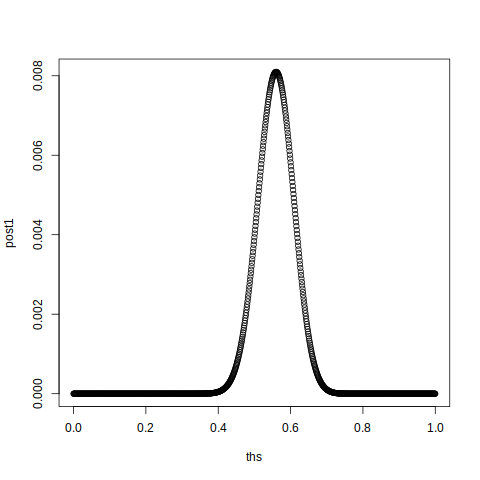
\includegraphics[width=.9\linewidth]{100.png}
\end{center}

\begin{verbatim}
plot(ths, post2)
\end{verbatim}

\begin{center}
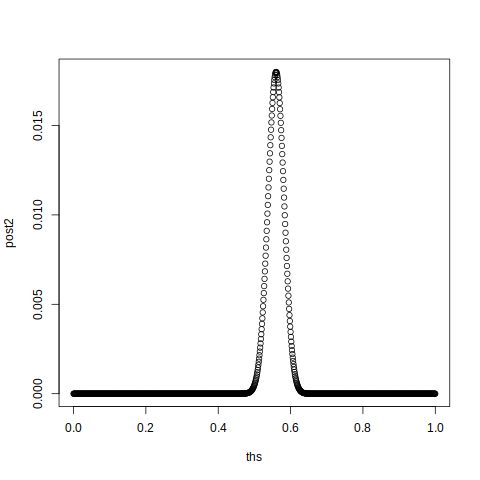
\includegraphics[width=.9\linewidth]{500.png}
\end{center}

\begin{verbatim}
plot(ths, post3)
\end{verbatim}

\begin{center}
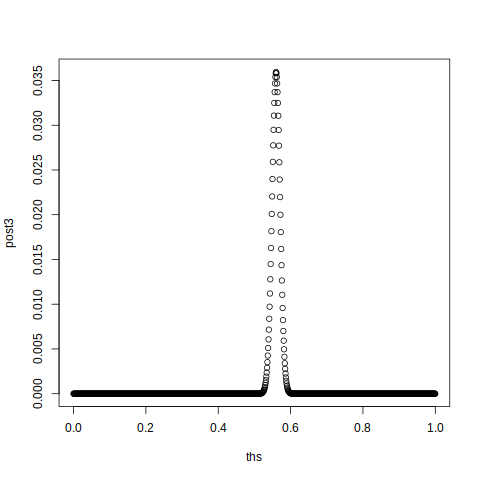
\includegraphics[width=.9\linewidth]{2000.png}
\end{center}


\subsection*{B)}
\label{sec:orgdc2f144}

\begin{verbatim}

cs1 <- cumsum(post1)
cs2 <- cumsum(post2)
cs3 <- cumsum(post3)

imin1  <- min((which(cs1 > .025)))
imin2  <- min((which(cs2 > .025)))
imin3  <- min((which(cs2 > .025)))


imax1  <- min((which(cs1 > .975)))
imax2  <- min((which(cs2 > .975)))
imax3  <- min((which(cs3 > .975)))


\end{verbatim}


\begin{verbatim}
cint1 <- ths[c(imin1,imax1)]
merr1 = cint1[2] - cint1[1] / 2
\end{verbatim}
\begin{verbatim}
0.422
\end{verbatim}

\begin{verbatim}
cint2 <- ths[c(imin2,imax2)]
merr2 = cint2[2] - cint2[1] / 2
\end{verbatim}

\begin{verbatim}
0.345
\end{verbatim}

\begin{verbatim}
cint3 <- ths[c(imin3,imax3)]
merr2 = cint3[2] - cint3[1] / 2
\end{verbatim}

\begin{verbatim}
0.324
\end{verbatim}

Margin of error decreases as \(n\) increases, ostensibly, because we are converging to the correct answer.
\end{document}